% Signal AC ou DC? Explications, schéma

En électronique, on utilise souvent la notion de signal pour décrire l'information qui est transportée le long des fils du circuit. Ce signal représente en fait la valeur du courant ou de la tension dans un fil au cours du temps. Il existe énormément de façons de caractériser ce signal. Une distinction importante est la notion de signal DC ou AC. Un signal DC (de l'anglais \textit{Direct Current}) correspond à une valeur qui reste constante au cours du temps. Inversement, un signal AC (\textit{Alternating Current}) correspond à un signal qui va osciller au cours du temps d'une valeur positive à une valeur négative. Par exemple, comme illustré à la Figure \ref{fig:ACDC}, la tension au borne d'une pile est dite DC car la tension est constante à 1.5V. Dans une prise de courant par contre, on retrouve une tension AC qui oscille de -310V à +310V, 50 fois par seconde.\\

\begin{figure}[!ht]
	\centering
	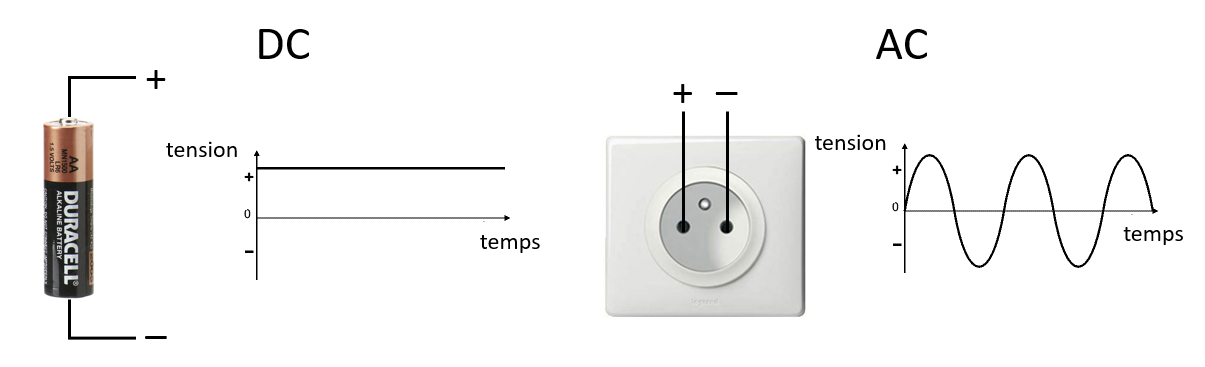
\includegraphics[width=\textwidth]{figures/AC-DC.PNG}
	\caption{Exemples de signaux DC et AC}
	\label{fig:ACDC}
\end{figure}

Dans le cas de notre micro, c'est encore un peu plus compliqué que cela. En effet, le signal produit par le micro reproduit les vibrations de l'air venant du son, et oscille donc bien comme un signal AC. Cependant, celui-ci est superposé à une tension DC (qui est due à l'électronique interne du micro, c'est un peu plus compliqué donc nous ne l'aborderons pas ici). Une illustration de ceci est présenté à la Figure \ref{fig:ACplusDC}, mais attention ce n'est pas à l'échelle!

\begin{figure}[!ht]
	\centering
	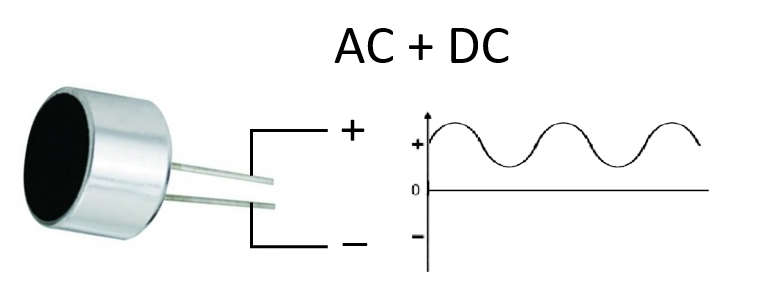
\includegraphics[width=.5\textwidth]{figures/microSignal.PNG}
	\caption{Signal AC superposé sur une tension DC}
	\label{fig:ACplusDC}
\end{figure}